

\chapter{Distributed GPU SpMV (incomplete)}
\label{chap:multigpu_rbffd}

Recent advances in distributed (multi-)GPU computing involve NVidia's GPU Direct technology. GPU Direct allows hardware like the PCI-e bus to directly access memory on the GPU device. CUDA V5.5 adds full support for MPI applications 



Lawlor \cite{Lawlor2009} wraps a subset of MPI collectives, memory copies between GPU and CPU, and---to some extent---callbacks to GPU kernels behind a simplified API called cudaMPI. Although the concept of cudaMPI is good for minimally invasive design, the library only provides a handful of  a limited subset of MPI  a for overlapping communication and computation.  

OpenCL does not support must be explicitly copied to the CPU 



%TODO: \cite{Goeddeke2009} \cite{Erez2007}

Distributing SpMV across multiple GPUs poses a new problem: as previous mentioned, the data sent and received via MPI collectives must be copied from device to host and vice-versa. To amortize this cost we introduce a novel overlapping algorithm to hide the cost of communication behind the cost of a concurrent SpMV on the GPU. 


Petascale computing centers around the world are leveraging GPU accelerators to achieve peak performance. In fact, many of today's high performance computing installations boast significantly more GPU accelerators than CPU counterparts. The Keeneland project is one such example, currently with 240 CPUs accompanied by 360 NVidia Fermi class GPUs with at least double that number expected by the end of 2012 \cite{Vetter2011}. 

Such throughput oriented architectures require developers to decompose problems into thousands of independent parallel tasks in order to fully harness the capabilities of the hardware. To this end, a plethora of research has been dedicated to researching algorithms in all fields of computational science. Of interest to us are methods for atmospheric- and geo-sciences. 


Similar approaches to overlapping communication and computation can be found in \cite{Schubert2011} and \cite{Thibault2009}.

When operating on multiple GPUs we avoid the copy-out or decode phase by requiring that the local ordering of nodes sort the set $\setDepend$ by the rank of the process sending each node. This way, when the MPI collective finishes and all values arrive contiguous by provider, the data can be copied directly to the GPU without reordering.

\section{Overlapping with the GPU}

Overlapping communication and GPU computation is enabled by two levels of asynchronous commands: 
\begin{itemize} 
\item \emph{Non-blocking MPI}. The MPI\_Isend/MPI\_Irecv routines are used to post communication and immediately return the main thread to computation. 
\item \emph{Asynchronous GPU Queues}. Two OpenCL queues are utilized to send commands to the GPU. 
\end{itemize}

 
\begin{figure} 
\centering
\begin{subfigure}{0.48\textwidth}
\centering
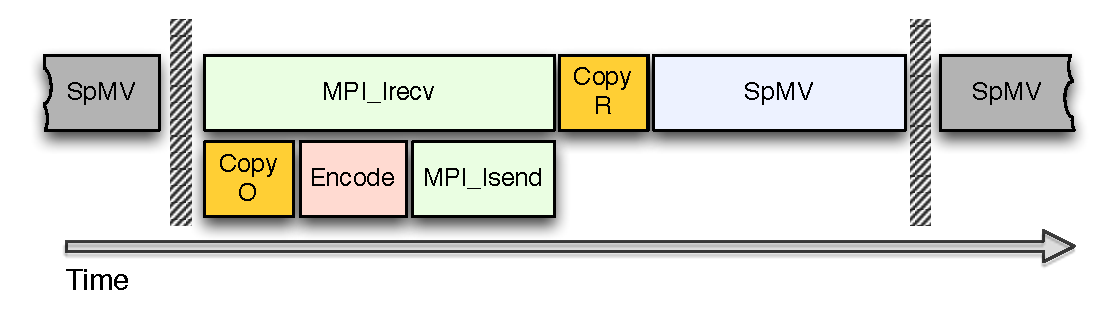
\includegraphics[width=\textwidth]{../figures/omnigraffle/GPU_IsendIrecv.pdf}
\caption{GPU and MPI\_Isend/MPI\_Irecv (Non-Overlapping)}
\label{fig:isendirecv_gpu}
\end{subfigure}
\quad
\begin{subfigure}{0.48\textwidth}
\centering
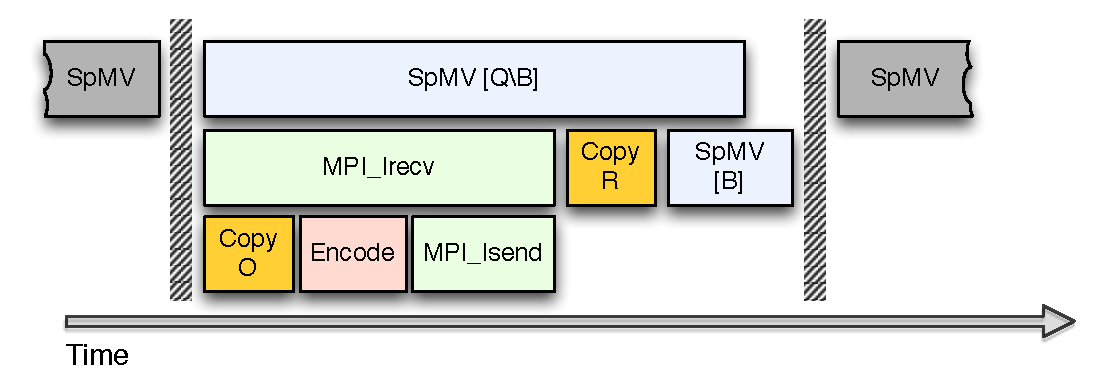
\includegraphics[width=\textwidth]{../figures/omnigraffle/GPU_OverlapGPU.pdf}
\caption{GPU and MPI\_Isend/MPI\_Irecv (Overlapping)}
\label{fig:overlap_gpu}
\end{subfigure}
\caption{Overlapping GPU kernels with CPU managed communication. Task block sizes are not drawn to scale.} 
\label{fig:gpu_mpi_tuning}
\end{figure}




\section{Distributed GPU Performance}


\subsection{Non-Overlapping Multi-GPU Results} 

See Appendices~\ref{app:keeneland_alltoallv_benchmarks} and \ref{app:spear_alltoallv_benchmarks} for scaling benchmarks from the non-ViennaCL multi-GPU implementation. Appendix~\ref{app:keeneland_alltoallv_benchmarks} demonstrates the scalability of an iteration of RK4 as applied in \S~\ref{sec:cosine_bell} on the Keeneland GPU cluster---the benchmark assumes three SpMV operations per intermediate evaluation of the RK4 time-step. Appendix~\ref{app:spear_alltoallv_benchmarks} is similar, but considers only two SpMV operations per evaluation corresponding to the test case in \S~\ref{sec:vortex_rollup}. In both cases, the performance is based on a non-overlapping communication collective (MPI\_Alltoallv).

Benchmarks


\subsection{Overlapping Results}
We scale the SpMV across the GPUs on Cascade.


By comparing benchmarks from the non-overlapped and overlapped GPU cases, we get the speedup: 
\begin{align*} 
S_p = \ ^{t_{non-overlapped}} /_{t_{overlapped}}
\end{align*}
in using the overlapped solution. Any reduction in time is evidence of overlap. 

%Calculating the percentage reduction is useful to consider. The benchmarks are not complete (i.e., the actual time to compute SpMV1 is unknown). However, the time spent in non-SpMV related tasks (e.g., data transfer, encoding, and communication) is known from the unoverlapped case. Therefore, given the time for the overlapped SpMV case, we can calculate the amount of overlap as 

If speedup greater than $p = (Compute Nodes * PPN)$ is achieved 

\begin{table}[h]
\centering
\caption{GFLOP/sec achieved by the distributed ELL SpMV on Cascade's M2070 GPUs, with MPI communication overlapping two GPU kernels. The SpMV computes derivatives over a 3-D regular grid of size $N=4096000$ nodes (i.e., $160^3$). Data reflects various combinations of stencil sizes, number of compute nodes and number of processes per node (PPN). Quantities in parentheses denote the speedup factors achieved by the overlapping algorithm over the non-overlapping approach for identical combinations of compute nodes, PPN, stencil size, etc. }
\label{tbl:cascade_m2070_overlap}
\begin{tabular}{c|c|c|c|c|c|c}
 \multicolumn{2}{c}{ } & \multicolumn{4}{|c|}{Observed GFLOP/sec (Speedup over Non-overlapped)} \\  \hline
Compute Nodes   &   PPN  &   n=17   &   n=31   &   n=50   &   n=101   \\ \hline
1   &   1   &   8.5 (1.0x)   &   8.4 (1.0x)   &   9.0 (1.0x)   &  --    \\
2   &   1   &   13.8 (2.3x)   &   13.0 (1.9x)   &   13.1 (2.0x)   &   13.5 (1.8x)   \\
4   &   1   &   13.1 (1.9x)   &   25.1 (2.8x)   &   24.6 (2.4x)   &   25.2 (1.9x)   \\
8   &   1   &   24.5 (2.0x)   &   33.2 (2.3x)   &   41.2 (3.4x)   &   53.6 (2.3x)   \\ \hline
1   &   2   &   11.3 (3.4x)   &   12.2 (3.0x)   &   12.1 (3.2x)   &   12.7 (3.0x)   \\
2   &   2   &   13.0 (3.0x)   &   22.9 (4.2x)   &   23.1 (3.6x)   &   24.5 (3.0x)   \\
4   &   2   &   25.1 (2.3x)   &   37.8 (4.1x)   &   50.1 (5.0x)   &   53.5 (3.8x)   \\
8   &   2   &   35.8 (2.2x)   &   38.3 (2.5x)   &   59.6 (2.7x)   &   87.6 (3.7x)   \\ \hline
1   &   4   &   14.1 (\textbf{4.3x})   &   22.5 (\textbf{5.1x})   &   24.4 (\textbf{5.4x})   &   24.4 (\textbf{4.4x})   \\
2   &   4   &   19.6 (2.4x)   &   32.0 (4.2x)   &   37.2 (3.9x)   &   50.8 (4.6x)   \\
4   &   4   &   27.5 (2.2x)   &   38.6 (3.0x)   &   57.0 (3.0x)   &   81.3 (4.5x)   \\
8   &   4   &   50.9 (2.9x)   &   61.6 (2.2x)   &   88.8 (3.2x)   &   130.8 (3.5x)  
\end{tabular} 
\end{table}

The total time required to compute the distributed SpMV for 1 node and 4 PPN is observed in the neighborhood of 80 ms for $n=50$ and the non-overlapping algorithm (i.e. without splitting $\setCenters \backslash \setBoundary$ and $\setBoundary$). Of those 80 ms, approximately 60 ms is spent performing non-computation tasks such as transferring from GPU down to CPU, encoding and sending data via MPI and then transferring back up to the GPU. The remaining 20 ms is all dedicated to performing the SpMV.

By introducing the overlapped GPU kernels, the total time for the distributed SpMV for $n=50$ (1 node, 4 PPN) drops to approximately 15 ms---25\% less than the SpMV-only portion of the non-overlapped approach. Since the non-computation tasks amount to only 12 ms in the overlapped case, our first conclusion is that overlapping hides 100\% of communication for the cases tested in Table~\ref{tbl:cascade_m2070_overlap}, as well as the entire SpMV for $\setBoundary$. 

Within each block of Table~\ref{tbl:cascade_m2070_overlap} we expect the GFLOP/sec to double by row. Obviously the strong scaling in the case of the GPU is not ideal when executing more than one PPN. However, for $n=50$ and 1 PPN we see super but on only 32 GPUs, and impeded by the I/O hub bottleneck, we manage to achieve 130 GFLOP/sec for $n=101$. Compare this to the GFLOP/sec scaling results on Itasca in Figure~\ref{fig:compare_strong_scaling_gflops_all_stencils} where 130 GFLOP/sec requires approximately 


Greater than 4x speedup (bold-faced in Table~\ref{tbl:cascade_m2070_overlap}) is possible due to a design flaw on Cascade: each compute node has four attached GPUs connected to the host via a shared I/O hub. Concurrent data transfers from multiple GPUs to host, or vice versa---as would occur while executing a synchronized, distributed SpMV---result in contention on the hub and serialization of transfers. Serialization effectively quadruples the total run-time for 4 PPN. By overlapping communication and computation we notice two effects: a) contention disappears (or is at least hidden by computation), and b) 


\section{Multiple Kernel Scheduling}
describe fermi's ability to schedule multiple kernels, what it means for our queues. 
%Do we need multiple queues, or just one that is non-blocking. How do we indicate we are done communicating if there is no queue to add markers to? 


\section{Future Work}

One of the problems with choosing to work in OpenCL is the fact that the standard offers the lowest common denominator of features from the various hardware vendors that support it. Many vendor specific features never make it into the language. 

Take for example GPUDirect, a technology introduced first CUDA v3.1 for NVidia hardware. GPUDirect allows direct access to GPU memory addresses from various sources including other GPUs. The technology allows GPUs to bypass copies to host memory en-route to another GPU on the same compute node. Combine GPUDirect with the new MPI aware features in CUDA v5.0 and data can pass directly from a GPU onto the infiniband fabric and up to another GPU \cite{NvidiaGPUMPI}. This type of feature may never be available in OpenCL. 

The new Kepler K20s allow both concurrent kernel execution and dynamic parallelism. Dynamic parallelism is a means of scheduling new kernel launches from within an exist kernel. In order to support this feature,

K20s also support CUDA 5.5 which introduces MPI aware CUDA. The nvcc compiler now detects MPI calls and routes data movement directly from InfiniBand to the GPU memory rather than making a stop on the host memory. This is only possible with GPUDirect (direct memory addressing) and dynamic parallelism (to spawn an MPI process from a kernel). 

Features like MPI-CUDA will are unlikely to be available in OpenCL in the future. NVidia is no longer leading or distributing the OpenCL libraries with their driver. NVidia only plans to support the OpenCL spec v1.1.


